\documentclass[11pt]{article}
\usepackage[margin=1in]{geometry}
\usepackage{amsmath}
\usepackage{amssymb}
\usepackage{graphicx}
\usepackage{hyperref}
\usepackage{booktabs}

\title{Counterfactual Cell World: A Controlled Testbed for Single-Cell Perturbation Prediction}
\author{Atila Vahedian}
\date{May 2026}

\begin{document}
\maketitle

\begin{abstract}
This note describes a small research system for predicting how a cell population changes under unseen perturbations. The first version uses a synthetic single-cell world with known regulatory structure, hidden combinatorial interventions, and distribution-level evaluation. The point is not to claim biological discovery. The point is to build a hard, inspectable counterfactual benchmark before moving to real Perturb-seq data.
\end{abstract}

\section{Problem}

For each condition, the model observes a source population $X \in \mathbb{R}^{n \times g}$, a perturbation vector $p \in \mathbb{R}^{g}$, a cell type $c$, a dose $d$, and a time value $t$. It predicts a target population $Y \in \mathbb{R}^{n \times g}$.

The difficult case is a held-out perturbation combination. The model may see single perturbations or other combinations during training, but it must predict the target distribution for a combination that was never directly observed.

\section{Model}

The model has four pieces:

\begin{enumerate}
  \item a signed learned gene interaction matrix $A$,
  \item a context encoder over population statistics, perturbation, cell type, dose, and time,
  \item a residual latent transition applied to source cells,
  \item a Gaussian decoder that predicts per-cell expression mean and variance.
\end{enumerate}

The objective is

\[
\mathcal{L}
= \mathrm{NLL}(Y \mid \mu, \sigma)
+ \lambda_{\mathrm{mmd}}\mathrm{MMD}(\mu, Y)
+ \lambda_{1}\lVert A \rVert_{1}
+ \lambda_{\mathrm{dag}} h(A).
\]

The likelihood term rewards cell-level accuracy. The MMD term rewards population-level agreement. The graph penalties keep the learned map sparse and discourage cyclic shortcuts.

\section{Synthetic World}

The simulator samples latent gene programs, cell-type offsets, sparse regulatory couplings, and perturbable genes. A target cell population is generated by integrating a nonlinear regulatory drift:

\[
x_{k+1}
= x_k + \Delta t\left[-0.32x_k
+ \alpha \tanh(x_k A^\top + b_c + 0.25p + 0.95pA^\top)\right] + \epsilon.
\]

The stronger indirect term makes direct expression shifting a weak baseline for held-out combinations.

\section{Current Result}

\begin{table}[h]
\centering
\begin{tabular}{lrrrr}
\toprule
method & MSE & MAE & MMD & gene corr. \\
\midrule
model & 0.0386 & 0.1422 & 0.1021 & 0.8714 \\
direct shift & 0.1090 & 0.2356 & 0.1711 & 0.7218 \\
mean shift & 0.1428 & 0.2692 & 0.1905 & 0.7271 \\
\bottomrule
\end{tabular}
\caption{Held-out combinatorial perturbation split from the checked synthetic run. Lower is better except gene correlation.}
\end{table}

\begin{figure}[h]
\centering
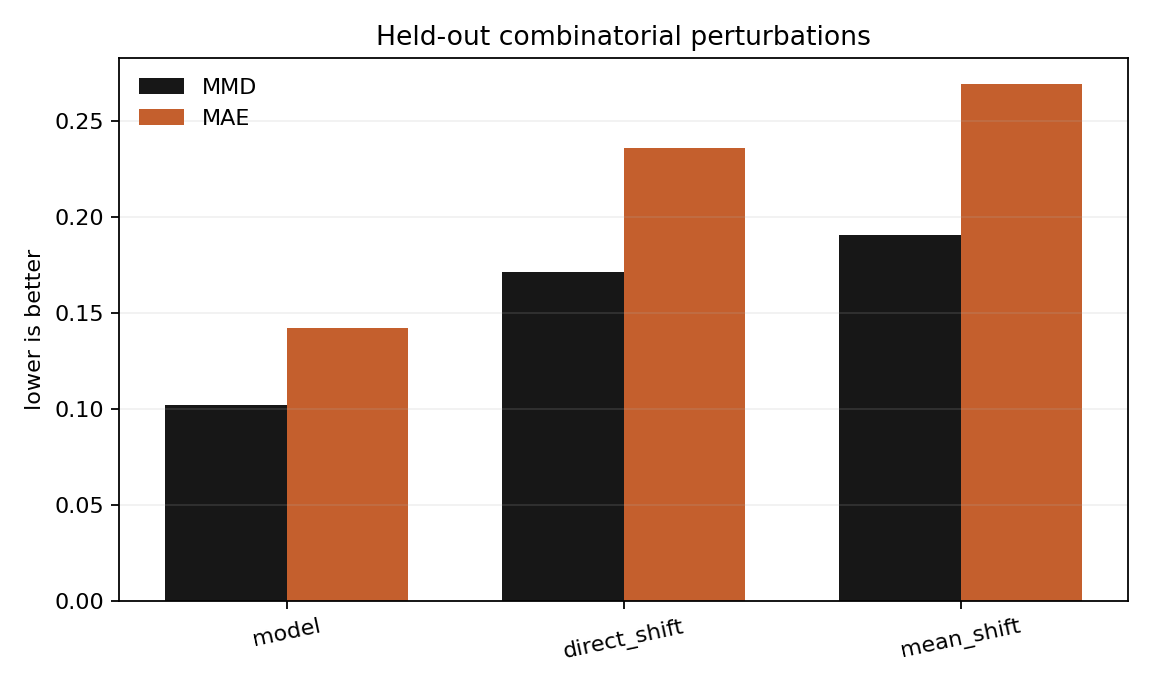
\includegraphics[width=0.95\linewidth]{../docs/figures/heldout_metrics.png}
\caption{Held-out metric comparison against two simple baselines.}
\end{figure}

\section{Next Step}

The next serious version should freeze a real Perturb-seq benchmark and report the same metrics by cell type, intervention order, dose, and unseen-gene setting. Public single-cell atlases are available through CELLxGENE, but atlas data and perturbation data should not be mixed casually because tissue, donor, assay, and batch effects can dominate the learning problem.

\end{document}
